\documentclass[border=3pt]{standalone}
% Preâmbulo compartilhado pelos diagramas TikZ da aula 5 de IHC (Processos de Design)
\usepackage[T1]{fontenc}
\usepackage[utf8]{inputenc}
\usepackage{lmodern}
\usepackage{amsmath}
\usepackage{xcolor}
\usepackage{tikz}
\usetikzlibrary{arrows.meta,angles,quotes,decorations.pathmorphing,calc,
                positioning,shapes.geometric,shapes.misc,backgrounds,fit,
                math}

% Paleta (mesma dos SVGs originais)
% Paleta da disciplina de IHC: acento roxo (#755099), da capa do livro.
% (o nome "dblue" é mantido para não alterar todos os diagramas)
\definecolor{dblue}{HTML}{755099}
\definecolor{dorange}{HTML}{B3541E}
\definecolor{dgreen}{HTML}{4A7C59}
\definecolor{dred}{HTML}{9C4B4B}
\definecolor{dcream}{HTML}{F4F1EA}
\definecolor{dshade}{HTML}{DDD7C9}

% Função gaussiana (não normalizada por padrão de escala visual)
\pgfmathdeclarefunction{gauss}{3}{%
  \pgfmathparse{1/(#3*sqrt(2*pi))*exp(-((#1-#2)^2)/(2*#3^2))}%
}

% Estilos comuns (prefixo d... para não colidir com chaves internas do pgf)
\tikzset{
  >={Stealth[length=2mm]},
  dguide/.style={gray!55, dashed, line width=0.4pt},
  daxis/.style={gray!60, line width=0.7pt, ->},
  dbody/.style={fill=black!3, draw=black!80, line width=1pt},
  dacc/.style={draw=dblue, line width=1pt},
  dlbl/.style={black!55, font=\small},
  dsub/.style={black!45, font=\footnotesize},
  dstate/.style={circle, draw=black!80, fill=dcream, line width=1pt,
                 minimum size=17mm, font=\large, inner sep=1pt},
  dobs/.style={circle, draw=black!80, fill=dshade, line width=1pt,
               minimum size=14mm, font=\large, inner sep=1pt},
  dbox/.style={rounded corners=2pt, draw=black!80, fill=dcream, line width=1pt,
               align=center, inner sep=6pt},
  dop/.style={circle, draw=black!80, fill=white, line width=1pt,
              minimum size=6mm, inner sep=0pt, font=\small},
  dtrans/.style={->, dblue, line width=1pt},
  dmeas/.style={->, dorange, line width=1pt},
  dcurve/.style={line width=1pt, dblue},
  dcurveb/.style={line width=1.4pt, dorange},
}

\begin{document}
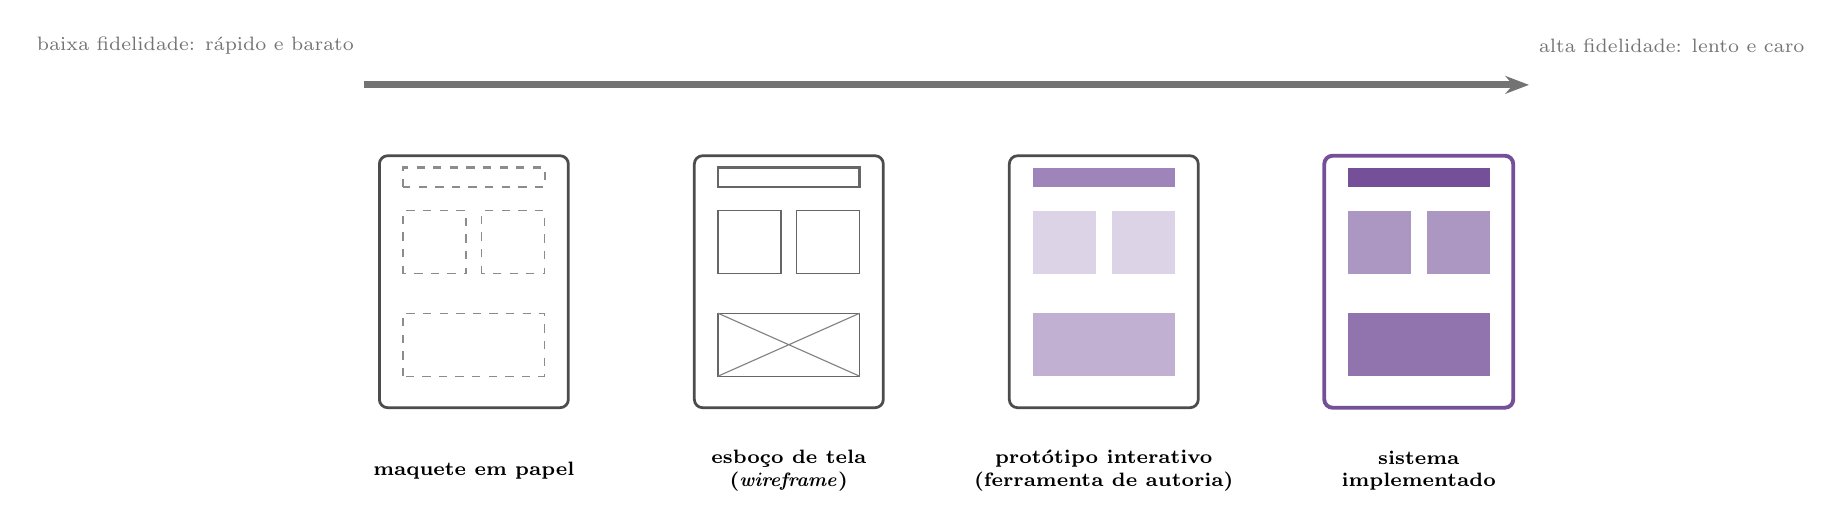
\begin{tikzpicture}[x=1cm,y=1cm,
   ph/.style={draw=black!70, line width=1pt, fill=white, rounded corners=3pt, minimum width=2.4cm, minimum height=3.2cm}]

  % 1 papel
  \node[ph] at (0,0) {};
  \draw[black!45, line width=0.8pt, dashed] (-0.9,1.2) rectangle (0.9,1.45); \draw[black!45, dashed] (-0.9,0.1) rectangle (-0.1,0.9); \draw[black!45, dashed] (0.1,0.1) rectangle (0.9,0.9); \draw[black!45, dashed] (-0.9,-1.2) rectangle (0.9,-0.4);
  \node[font=\scriptsize\bfseries, align=center] at (0,-2.4) {maquete em papel};
  % 2 wireframe
  \node[ph] at (4.0,0) {};
  \draw[black!60, line width=0.9pt] (3.1,1.2) rectangle (4.9,1.45); \draw[black!60] (3.1,0.1) rectangle (3.9,0.9); \draw[black!60] (4.1,0.1) rectangle (4.9,0.9); \draw[black!60] (3.1,-1.2) rectangle (4.9,-0.4);
  \draw[black!50] (3.1,-1.2) -- (4.9,-0.4) (3.1,-0.4) -- (4.9,-1.2);
  \node[font=\scriptsize\bfseries, align=center] at (4.0,-2.4) {esboço de tela\\(\textit{wireframe})};
  % 3 interativo
  \node[ph] at (8.0,0) {};
  \fill[dblue!70] (7.1,1.2) rectangle (8.9,1.45); \fill[dblue!25] (7.1,0.1) rectangle (7.9,0.9); \fill[dblue!25] (8.1,0.1) rectangle (8.9,0.9); \fill[dblue!45] (7.1,-1.2) rectangle (8.9,-0.4);
  \node[font=\scriptsize\bfseries, align=center] at (8.0,-2.4) {protótipo interativo\\(ferramenta de autoria)};
  % 4 código
  \node[ph, draw=dblue, line width=1.4pt] at (12.0,0) {};
  \fill[dblue] (11.1,1.2) rectangle (12.9,1.45); \fill[dblue!60] (11.1,0.1) rectangle (11.9,0.9); \fill[dblue!60] (12.1,0.1) rectangle (12.9,0.9); \fill[dblue!80] (11.1,-1.2) rectangle (12.9,-0.4);
  \node[font=\scriptsize\bfseries, align=center] at (12.0,-2.4) {sistema\\implementado};

  \draw[-{Stealth[length=3mm]}, black!55, line width=2.6pt] (-1.4,2.5) -- (13.4,2.5);
  \node[dlbl, font=\scriptsize, anchor=east] at (-1.4,3.0) {baixa fidelidade: rápido e barato};
  \node[dlbl, font=\scriptsize, anchor=west] at (13.4,3.0) {alta fidelidade: lento e caro};

\end{tikzpicture}
\end{document}
